\part{Statistiken}

Hier ein Überblick über die Codemenge:
\begin{center}
	\begin{tabular}{| l | l | l | l | l |}
		\hline
		& Dateien & Leerzeilen & Kommentare & Code \\ \hline
		main & 108 & 2253 & 3841 & 9467 \\ \hline
		test & 39 & 1358 & 184 & 6768 \\ \hline
		total & 147 & 3611 & 4025 & 16235 \\ \hline
	\end{tabular}
\end{center}

Damit macht der Testcode rund 42 Prozent des gesamten Codes aus.

Hier ein Überblick über die Testabdeckung:

\begin{figure}[H]
	\centering
	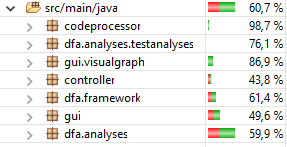
\includegraphics[width=0.8\textwidth]{Statistiken/coverage.png}
	\label{fig1}
\end{figure}


Hier wird lediglich die Abdeckung durch automatische Tests dargestellt. Zusätzlich dazu wurden noch manuelle Tests ausgeführt. Für diese stehen aber keine Überdeckungs-Statistiken zur Verfügung.